\documentclass[12pt]{article}

\usepackage{booktabs}% http://ctan.org/pkg/booktabs
\usepackage[utf8]{inputenc}
\usepackage{changepage}
\usepackage{pgfplots}
\usepackage{amssymb}
\usepackage{xcolor}
\usepackage{hyperref}
\usepackage{listings}
\usepackage[T1]{fontenc}
\usepackage[utf8]{inputenc}
\usepackage{adjustbox}
\usepackage{amsmath}
\usepackage{mathtools}
\usepackage{biblatex}
\usepackage{algorithm2e}
\RestyleAlgo{ruled}
\SetKwProg{Proc}{Procedure}{:}{}


\lstset{
  language=Python,
  numbers=left,
  numberstyle=\tiny,
  stepnumber=1,
  numbersep=5pt,
  tabsize=4,
  basicstyle=\ttfamily,
  columns=fullflexible,
  keepspaces,
}
\hypersetup{
    colorlinks,
    citecolor=black,
    filecolor=black,
    linkcolor=black,
    urlcolor=black
}

% Set page size and margins
% Replace `letterpaper' with `a4paper' for UK/EU standard size
\usepackage[letterpaper,top=2cm,bottom=2cm,left=3cm,right=3cm,marginparwidth=1.75cm]{geometry}

% Useful packages
\usepackage{amsmath}
\usepackage{mathtools}
\usepackage{graphicx}
\newenvironment{para}{\begin{adjustwidth}{13mm}{}}{\end{adjustwidth}}

\newcommand\tab[1][1cm]{\hspace*{#1}}

\newcommand{\tabitem}{\llap{\textbullet}}
\newcommand{\Hsquare}{%
\text{\fboxsep=-.2pt\fbox{\rule{0pt}{1ex}\rule{1ex}{0pt}}}%
}

\newtheorem{Definizione}{Definizione}[subsection]
\newtheorem{Lemma}{Lemma}[subsection]
\newtheorem{Teorema/Definizione}{Teorema/Definizione}[subsection]
\newtheorem{Corollario}{Corollario}[subsection]
\newtheorem{Teorema}{Teorema}[subsection]
\newtheorem{Proposizione}{Proposizione}[subsection]
\newtheorem{Notazione}{Notazione}[subsection]
\newtheorem{Commento}{Commento}[subsection]
\newtheorem{Dimostrazione}{Dimostrazione}[subsection]
\newtheorem{Osservazione}{Osservazione}[subsection]
\newtheorem{Nota}{Nota}[subsection]

\DeclarePairedDelimiter\ceil{\lceil}{\rceil}
\DeclarePairedDelimiter\floor{\lfloor}{\rfloor}


\title{Introduzione all'intelligenza artificiale}
\author{spitfire}
\date{A.A. 2024-2025}
\begin{document}
\begin{figure}
    \centering
    
\includegraphics[width=0.35\textwidth]{Images/Logo scienze bicocca.png}
\end{figure}

\vspace{10cm}
\date{A.A. 2024-2025}


\maketitle

\newpage

\tableofcontents
\newpage

\section{Introduzione}
Che cos'è l'intelligenza artificiale? Prima di tutto, dovremmo definire che cos'è \textbf{l'intelligenza}.
Negli anni sono state date molte definizioni:
\begin{itemize}
    \item "L'intelligenza è una capacità mentale molto \textbf{generale} che, tra le altre cose, coinvolge la capacità di \textbf{ragionare, pianificare, risolvere problemi, pensare in maniera astratta, comprende idee complesse, apprendere velocemente e imparare dall'esperienza}".
     da "Mainstream science on intelligence: An editorial with 52 signatories, history,
        and bibliography, Intelligence 24(1):13–23, 1997"
    \item "L'intelligenza è la \textbf{capacità di adattarsi efficacemente all'ambiente}, o cambiando se stessi o cambiando l'ambiente oppure trovandone uno nuovo... l'intelligenza non è un singolo processo mentale, ma piuttosto una combinazioni molti processi mentali indirizzati verso un adattamento efficace all'ambiente" da Encyclopedia Britannica, 2006.
    \item ... 
\end{itemize}
Quindi il problema di fondo è quello di \textbf{definire l'intelligenza}. Le relazioni tra l'informatica e le scienze cognitive non sono quindi
sporadici e sono particolarmente significativi. Uno schema proposto da \textbf{Russel e Norvig e il seguente}:
\begin{center}
    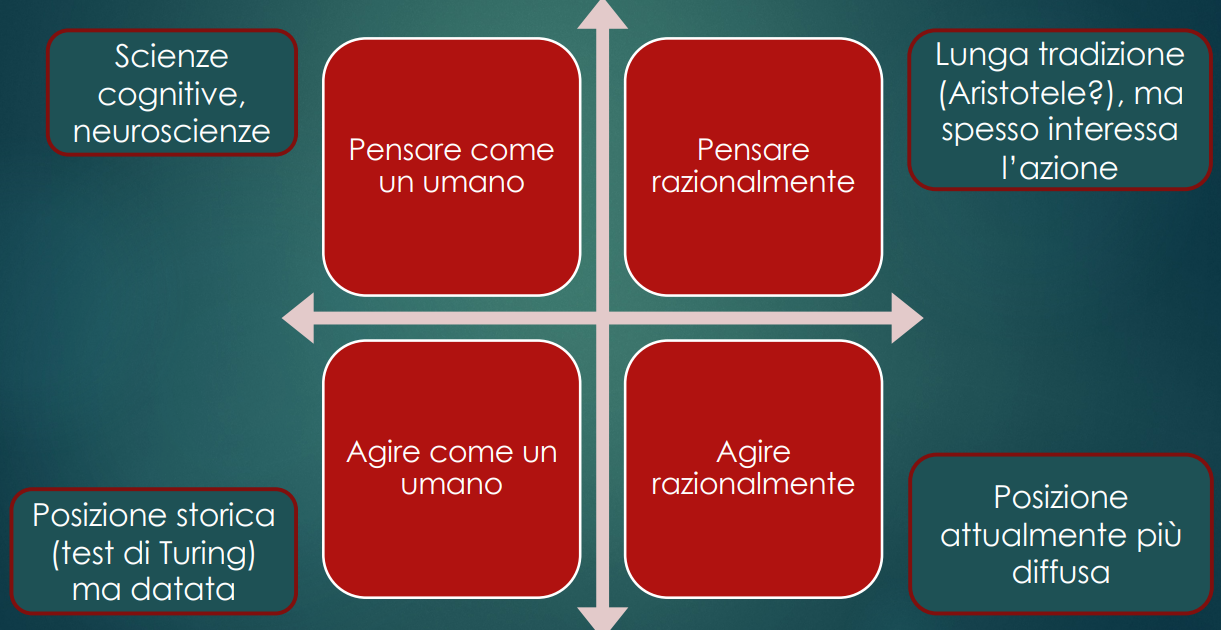
\includegraphics[width = 1\linewidth]{Images/1.PNG}
\end{center}
essi propongono uno schema che "astrae" i tipi di intelligenza, ponendoli su due dimensioni:
\begin{itemize}
    \item Sull'asse delle ordinate troviamo il contrasto tra \textbf{l'imitare l'essere umano} (cioè imitare il suo modo di agire) e il \textbf{pensare come un umano} (quindi il "risolvere problemi")
    \item Sull'asse delle ascisse troviamo il \textbf{contrasto tra il pensare e l'agire}
\end{itemize}
\subsection{Storia dell'intelligenza artificiale}
Il termine "intelligenza artificiale" fu coniato nell'agosto del 1955 da \textbf{John McCarty, Marvin Minsky, Allan Newell e Herbert Simon}, i quali proposero al Dartmouth College di Hanover (New Hampshire) di organizzare il "Dartmouth College Summer Research Project on Artificial Intelligence"; cioè uno spazio
dove accogliere persone che volessero discutere del tema dell'intelligenza artificiale. Essi descrissero l'iniziativa nel seguente modo:
\begin{center}
    "Lo studio dovrà procedere sulla base della congettura che ogni aspetto dell'apprendimento o ogni altra caratteristica dell'intelligenza può essere sia, in linea di principio, descrivibile in maniera talmente precisa che una macchina può essere costruita per simularla"
\end{center} 
In realtà, la storia dell'intelligenza artificiale risale persino ad Alan Turing (1912-1954), il quale definì il cosiddetto \textbf{Test di Turing}: l'idea di questo test è che ci sia un essere umano $C$ separato fisicamente da due interlocutori, uno anch'esso umano, chiamato $B$, e l'altro una macchina, chiamata $A$, programmata in qualche modo.
$C$ non può interloquire direttamente con $A$ e $B$, tuttavia può scambiare messaggi con essi tramite un qualche sistema di comunicazione (foglietti di carta, una chat ecc...). Quando $C$, interagendo in maniera dialogica con i due interlocutori, non riesce più di una certa percentuale di volte a capire chi dei due è la macchina allora $A$ mostra un
comportamento intelligente (cioè "agisce come un essere umano", "agisce razionalmente").
\begin{center}
    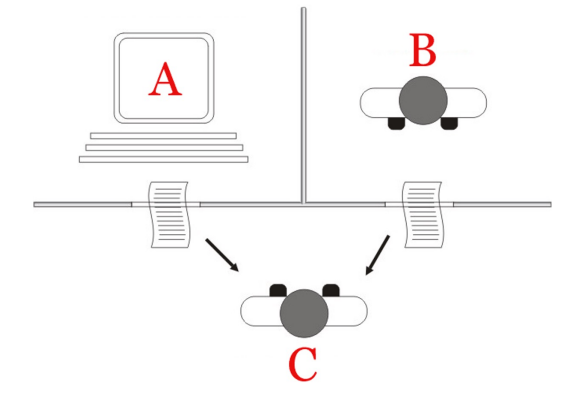
\includegraphics[width = 0.50\linewidth]{Images/2.PNG}
\end{center}
Tuttavia, nel 1966, fu prodotto un programma chiamato \textbf{ELIZA}, il quale imitava uno \textbf{psicoterapeuta}, che \textbf{superò il test di Turing nonostante fosse basato su regole di pattern matching con espressioni regolari}. Il programma portava l'utente ad avere una
\textbf{conversazione plausibile}, cioè davano all'utente l'illusione di star parlando con un \textbf{essere umano}. Per questo, il test di Turing ha solo un \textbf{interesse storico} e risulta poco interessante.
Non è quindi un caso che, nel gruppo di studio citato sopra, una delle cose di cui ci si è occupati non fosse dedicata subito all'apprendimento ma al \textbf{ragionamento}.
\subsection{Approcci simbolici}
La disciplina che si occupa delle forme corrette di ragionamento è la \textbf{logica}.
La logica è quindi lo studio sistematico delle \textbf{forme di inferenza valida}, cioè forme di elaborazione e rappresentazione della conoscenza
che garantiscono che da informazioni vere si derivino informazioni vere.
La \textbf{logica computazionale} è l'uso della logica per effettuare ragionamenti riguardo alla computazione (es. dimostrazione della correttezza di un programma).
Alcuni sforzi iniziali nel settore dell'intelligenza artificiale erano legati alla realizzazione di \textbf{dimostratori automatici di teoremi}. \newline 
Un'\textbf{inferenza} è un ragionamento che stabilisce delle relazioni tra \textbf{premesse} e delle \textbf{conclusioni}. I \textbf{modelli computazionali} di inferenza si interessano quindi di:
\begin{itemize}
    \item Quali informazioni possono trarre dato un insieme di premesse?
    \item Perché la conclusione è corretta?
\end{itemize}
L'inferenza riguarda quindi il trarre delle conclusioni quando \textbf{le premesse sono vere}.
Dire che un'inferenza è corretta, tuttavia, \textbf{non dice nulla sul valore di verità delle conclusioni}, quindi un ragionamento può essere corretto anche se \textbf{le premesse sono false}.
Le varie forme di inferenza sono:
\begin{itemize}
    \item \textbf{Deduzione}:"Se le premesse sono vere, allora le conseguenze devono essere anch'esse vere". Questa forma di ragionamento parte da delle premesse \textbf{generali} e trae delle conclusioni \textbf{particolari}
    \item \textbf{Inferenze di "senso comune"}: Esse non sono sempre "valide", ma sono \textbf{utili nella pratica}; sono modelli per spiegare \textbf{quando un inferenza è giustificata} e calcolarla di conseguenza. Esempi di questo tipo di inferenze sono:
    \begin{itemize}
        \item \textbf{Induzione}: Questa forma di ragionamento parte da delle \textbf{osservazioni particolari} e arriva a delle \textbf{conclusioni generali}.
        \item \textbf{Abduzione}: Sillogismo in cui la premessa maggiore è certa e la premessa minore è probabile, per cui anche la conclusione risulta solo probabile.
    \end{itemize}
\end{itemize}
Dove si applica quindi l'IA di tipo simbolico?
\begin{itemize}
    \item Problemi che possono essere espressi in termini di \textbf{vincoli} che devono essere soddisfatti
    \item Situazioni in cui si devono studiare delle \textbf{sequenze di azioni} per portare un certo stato dell'ambiente circostante ad un determinato obbiettivo
\end{itemize}
In passato, si svilupparono applicazioni il cui obbiettivo era \textbf{risolvere problemi specifici e delimitati}; questa applicazioni presero il nome di \textbf{sistemi esperti}.
Degli esempi notevoli sono:
\begin{itemize}
    \item \textbf{Dendral}(Anni '60): Automatizzò il processo di decisione e l'approccio alla risoluzione dei problemi dei chimici organici
    \item \textbf{Mycin}(Anni '70): Supportò  l'identificazione dei batteri che causavano infezioni gravi e la raccomandazione di antibiotici 
\end{itemize}
\begin{center}
    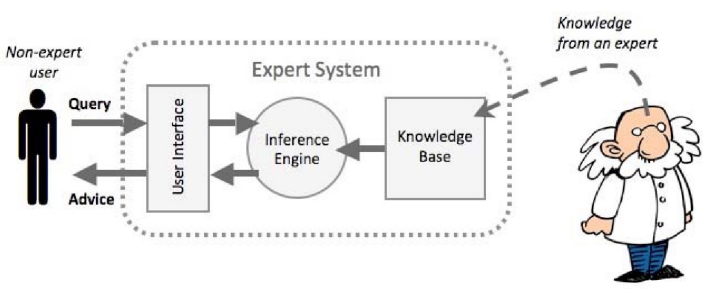
\includegraphics[width = 0.80\linewidth]{Images/3.PNG}
\end{center}
Tuttavia, presto divennero evidenti i \textbf{limiti} dei sistemi esperti:
\begin{itemize}
    \item È necessario trovare un \textbf{esperto disposto a codificare la sua conoscenza all'interno della base di conoscenza}
    \item I sistemi esperti \textbf{non scalano bene con grandi quantità di informazioni}: l'aggiornamento del sistema esperto rispetto ai \textbf{nuovi approcci alla risoluzione del problema per cui è stato costruito} è particolarmente complesso, sopratutto se il problema \textbf{non è ben delimitato}. La base di conoscenza del sistema rischierebbe quindi di \textbf{contenere troppi assiomi e regole}.
    \item Il costo di sviluppo di questi sistemi è \textbf{elevato}
\end{itemize}
\subsection{Approcci sub-simbolici}
I sistemi di IA \textbf{sub-simbolici} \textbf{non manipolano una rappresentazione simbolica} per trovare soluzioni a problemi, ma effettuano \textbf{calcoli secondo alcuni principi} che hanno dimostrato di essere in grado di portare alla risoluzione del problema.
Esempi notevoli sono:
\begin{itemize}
    \item Algoritmi genetici
    \item Reti Neurali
    \item "Intelligenza dello sciame" (Swarm Intelligence)
\end{itemize}
Tuttavia, l'argomento più importante correntemente è quello del \textbf{Machine Learning}.
Le \textbf{reti neurali artificiali} (Artificial Neural Networks (ANN)) sono una simulazione astratta del nostro sistema nervoso, il quale
contiene una collezione di \textbf{neuroni} che comunicano tra loro tramite delle connessioni dette \textbf{assoni}.
\begin{center}
    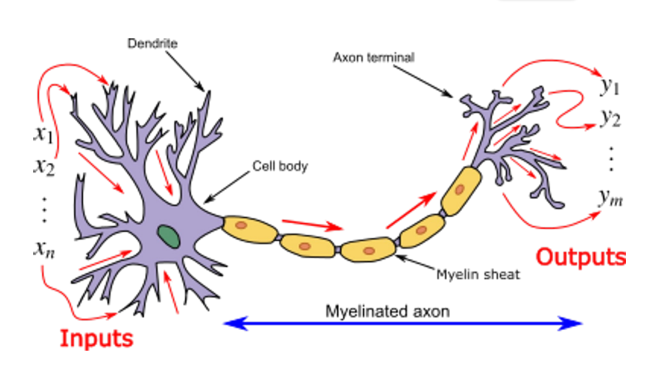
\includegraphics[width = 0.60\linewidth]{Images/4.PNG}
\end{center}
Il modello delle ANN ha delle certe somiglianze con gli assoni e i dendriti nel nostro sistema nervoso.
Il primo modello di rete neurale artificiale fu proposto nel 1943 da \textbf{McCulloch} e \textbf{Pits} nei termini di un \textbf{modello computazione dell'attività neurale}.
Questo modello fu poi seguito da altri modelli proposti da \textbf{John Von Neumann, Marvin Minsky, Frank Rosenblatt} e molti altri.
Rosenblatt definì un modello "algebrico" del neurone, chiamato \textbf{percettrone}; esso è una pietra miliare della ricerca sulle reti neurali.
Il percettrone cerca di \textbf{simulare le operazioni svolte da un singolo neurone}; l'apprendimento quindi diventa un problema di \textbf{scegliere i pesi e le soglie corrette}.
\begin{center}
    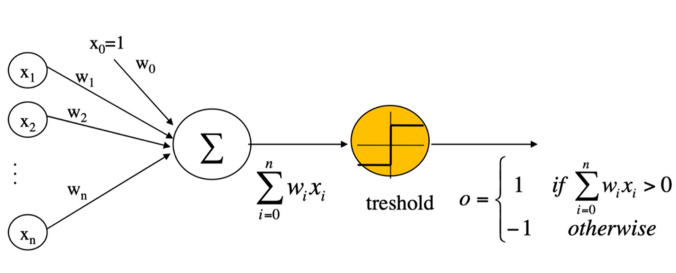
\includegraphics[width = 0.70\linewidth]{Images/5.PNG}
\end{center}
tendenzialmente, si arriva ad avere dei \textbf{percettroni multistrato}, dove ogni nodo è un singolo percettrone (introdotti per la prima volta da Minksy e S.Papert nel 1969)
\begin{center}
    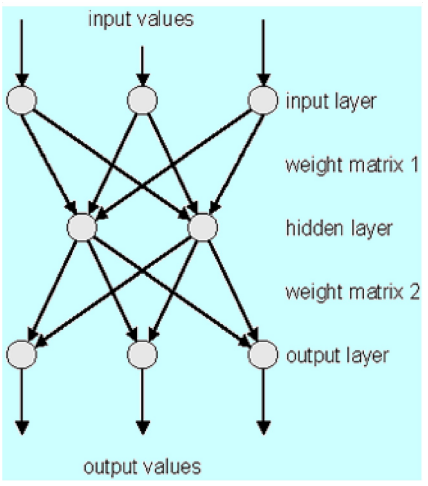
\includegraphics[width = 0.40\linewidth]{Images/6.PNG}
\end{center}
come faccio però a determinare i pesi di tutta la rete? Si utilizza il meccanismo della \textbf{back-propagation}: l'idea è che l'input è una \textbf{rappresentazione del problema} e che vi sia un \textbf{output desiderato} che la rete deve offrire;
inizialmente la rete neurale ha \textbf{dei pesi causali}, che verranno corretti \textbf{retropropagando} l'output desiderato sulla rete.
Questo è un approccio all'apprendimento che si dice "\textbf{supervisionato}".
\begin{center}
    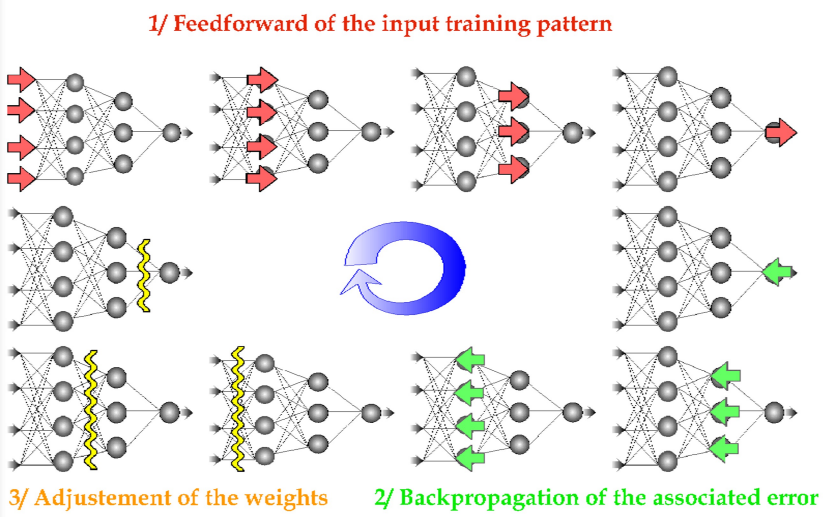
\includegraphics[width = 0.75\linewidth]{Images/7.PNG}
\end{center}
Oltre all'apprendimento supervisionato, esistono molte altre tecniche di addestramento:
\begin{center}
    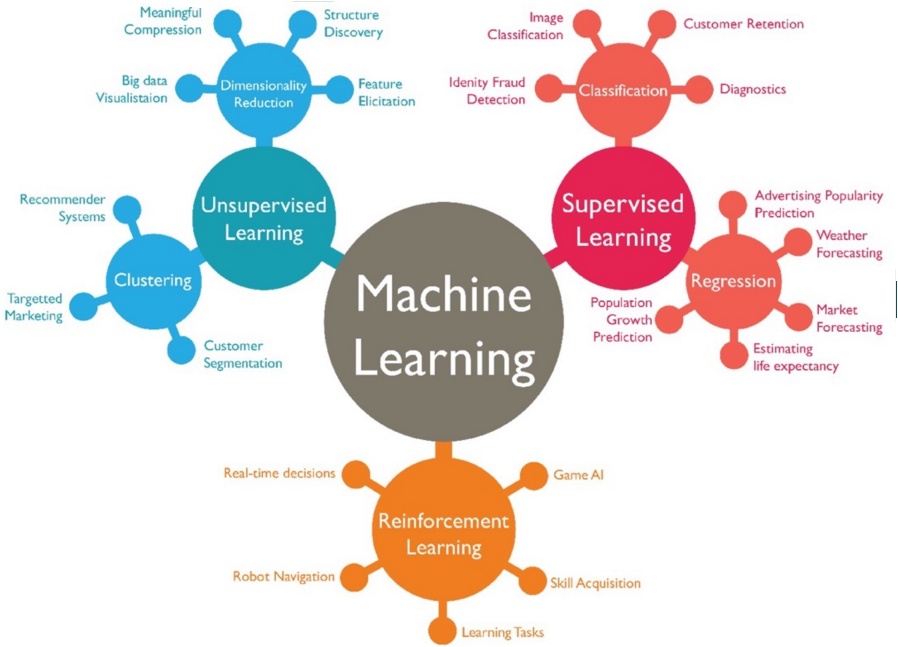
\includegraphics[width = 0.95\linewidth]{Images/8.PNG}
\end{center}
\newpage
\subsection{Agenti intelligenti, architetture e ambienti}
Un \textbf{agente} è tutto ciò che può essere vista come "percepente il suo ambiente" attraverso dei \textbf{sensori} e che può \textbf{agire su tale ambiente} attraverso degli \textbf{attuatori}.
Come agenti possono essere quindi classificati
\begin{itemize}
    \item Gli \textbf{esseri umani}, definendo come "sensori" gli occhi, le orecchie ecc... e come attuatori la bocca, le gambe, le braccia ecc...
    \item Gli \textbf{agenti robotici}, i quali hanno telecamere e sensori ad infrarossi come sensori e vari motori come attuatori
    \item Nulla vieta che \textbf{un agente possa essere anche solamente un software}
\end{itemize} 
Un agente è quindi rappresentabile nel seguente modo:
\begin{center}
    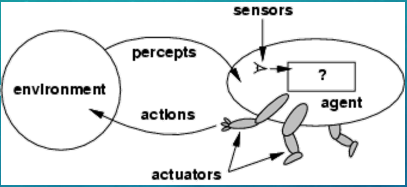
\includegraphics[width = 0.45\linewidth]{Images/9.PNG}
\end{center}
la forma più generale di agente è una \textbf{funzione} che mappa \textbf{l'insieme potenza di tutte le percezioni istantanee $\mathcal{P}^*$} ad una azione dell'insieme \textbf{di tutte le azioni eseguibili dall'agente} $\mathcal{A}$, cioè:
$$f: \mathcal{P}^* \rightarrow \mathcal{A}$$
quindi, l'agente può mappare una \textbf{sequenza arbitrariamente lunga di percezioni istantanee} (insieme potenza di $\mathcal{P}$) \textbf{ad una singola azione contenuta nell'insieme $\mathcal{A}$}.
Un agente è quindi \textbf{la sua architettura (la sua struttura profonda) più il suo programma (specifico dell'agente)}.
Gli agenti possono essere classificati, in base alla loro architettura interna, nelle seguenti classi:
\begin{itemize}
    \item Agenti con riflessi semplici
    \item Agenti con riflessi basati su un modello
    \item Agenti basati su un obbiettivo e su un modello
    \item Agenti basati su un'utilità e un modello.
\end{itemize}
\subsubsection{Agenti con riflessi semplici}
Un agente con riflessi semplici è un agente in cui vi è una comunicazione con l'ambiente (tramite i sensori e gli attuatori dell'agente).
Al suo interno, i sensori vanno a realizzare una "vista" che rappresenta \textbf{lo stato attuale dell'ambiente circostante}.
L'agente deve quindi \textbf{scegliere quale azione intraprendere} e, in questo caso, per farlo ha solamente a disposizione delle regole del tipo
\textbf{condizione-azione}.
\begin{center}
    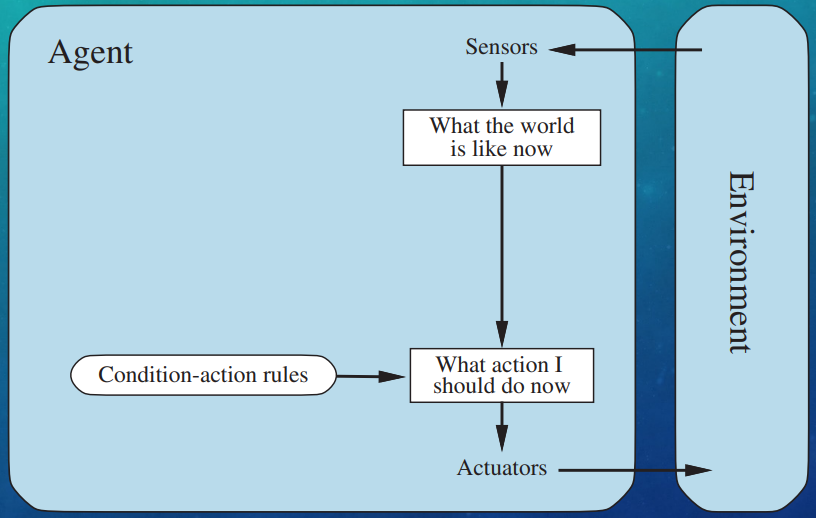
\includegraphics[width = 0.70\linewidth]{Images/10.PNG}
\end{center}
questo tipo di agente è \textbf{privo di stato}. Con architetture estremamente semplici, magari con più agenti, si riescono
quindi ad ottenere dei comportamenti, se non intelligenti, perlomeno utili.
\subsubsection{Agenti con riflessi basati su modello}
\begin{center}
    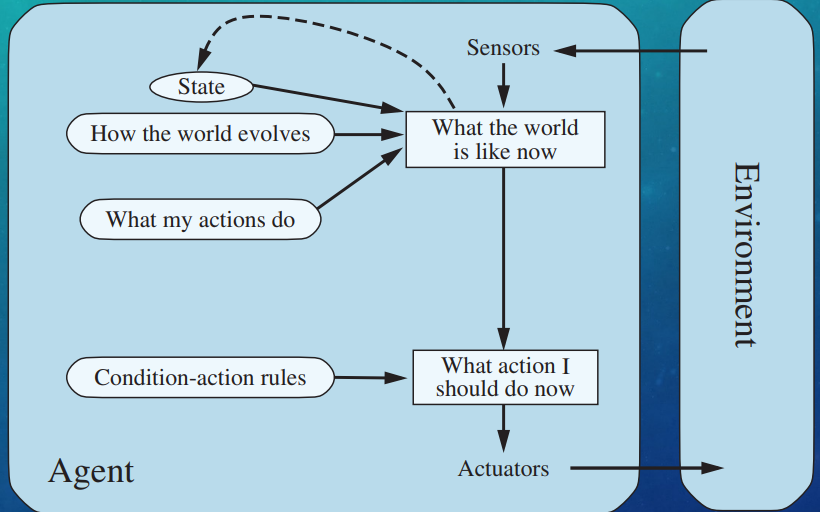
\includegraphics[width = 0.70\linewidth]{Images/11.PNG}
\end{center}
La differenza più significativa di questi agenti rispetto agli agenti con riflessi semplici è la \textbf{conoscenza del proprio stato interno}.
Questo tipo di agente può quindi \textbf{riflettere sul proprio stato} e quindi effettuare azioni basate su di esso.
Anche ignorando che l'ambiente ha una struttura, questo tipo di agente deve quindi avere un \textbf{modello matematico dell'evoluzione del mondo rispetto alle azioni fatte} che gli permetta
di decidere quale azioni intraprendere. Lo stato \textbf{non è una memoria che mantiene lo stato del mondo}, ma è solo un'informazione sullo stato dell'agente.
L'agente, inoltre, deve \textbf{poter percepire il proprio stato come parte dell'ambiente} (o come una "percezione esterna" o proprio come uno stato interno all'agente e che esso aggiorna e conosce).
Questo tipo di agente quindi può eseguire \textbf{comportamenti più adattivi rispetto all'ambiente}.
\subsubsection{Agenti basati su un obbiettivo e su un modello}
\begin{center}
    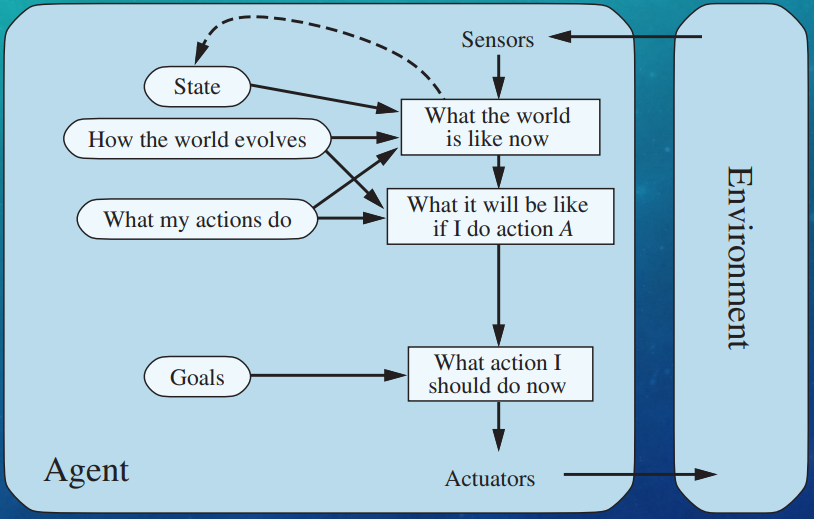
\includegraphics[width = 0.70\linewidth]{Images/12.PNG}
\end{center}
Questo tipo di agente, tramite i sensori ed eventualmente l'informazione di stato, si fa un'idea dello stato in cui si trova.
Questo agente presenta una \textbf{funzione che, partendo dallo stato dell'agente, ritorna tutte le azioni ammissibili che l'agente può intraprendere}.
Lo stato attuale viene quindi messo come \textbf{radice di un albero} e generiamo, a partire da esso, un numero di figli pari al numero di azioni ammissibili.
Possiamo costruire questo albero perché sappiamo \textbf{in quale stato si andrà a finire eseguendo una determinata azione}.
Per ogni nodo di stato che viene generato in questo modo, potremmo generare \textbf{un ulteriore livello di approfondimento dell'albero}, cioè ogni nodo stato potrebbe diventare la radice di un ulteriore sotto-albero.
In linea di principio, potrei quindi costruire l'albero di \textbf{tutti gli stati raggiungibili possibili tramite ogni combinazione possibile di azioni}.
Ovviamente, il fattore di ramificazione di questo albero è \textbf{estremamente elevato}. L'agente deve quindi esplorare questo albero per capire se esistono delle configurazioni nelle quali \textbf{l'obbiettivo sia verificato}.
Vi è quindi una \textbf{costruzione dello spazio degli stati} e una \textbf{ricerca nello spazio degli stati}. \newline
Per capire quali azioni intraprende, l'agente deve quindi risolvere un \textbf{problema di ricerca}, il quale consiste in:
\begin{itemize}
    \item Uno \textbf{spazio degli stati}
    \item Una \textbf{funzione di successione}, che dato un certo stato e l'azione che si vuole intraprendere (la quale potrebbe avere un certo \textbf{costo}), in quale stato si vada a finire. Questa funzione mi dice anche \textbf{quali sono le azioni ammissibili in un determinato stato}
    \item Uno \textbf{stato iniziale}
    \item Una \textbf{funzione "goal test"} che ci dica \textbf{se l'obbiettivo è stato raggiunto o meno}
\end{itemize}
Una \textbf{soluzione} ad un problema di ricerca è una \textbf{sequenza di azioni} (un piano) che trasformano lo stato iniziale nello stato obbiettivo.
Uno \textbf{spazio di ricerca} astrae l'ambiente per selezionare solo le informazioni utili per risolvere il problema.
\begin{center}
    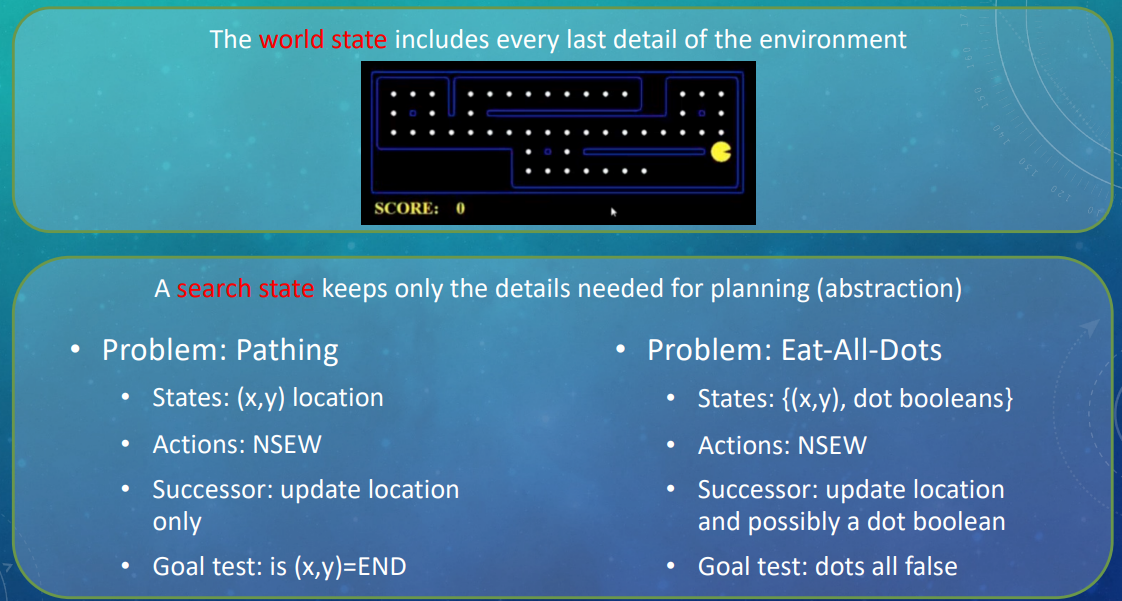
\includegraphics[width = 1\linewidth]{Images/13.PNG}
\end{center}
lo spazio degli stati, per problemi di ragionevole complessità, \textbf{tendono ad esplodere}, quindi non si possono applicare generalmente algoritmi \textbf{forza bruta} per trovare una configurazione che risolva il problema.
La costruzione dello spazio di ricerca avviene tramite \textbf{un albero di ricerca}, dove:
\begin{itemize}
    \item Lo stato iniziale è il nodo radice
    \item I figli corrispondono agli stati successivi data un'azione
    \item I nodi mostrano gli stati, ma \textbf{corrispondono ai piani per raggiungere quelli stati}
    \item Per la maggior parte dei problemi, non arriviamo mai a costruire l'intero albero (troppo grande)
\end{itemize}
\begin{center}
    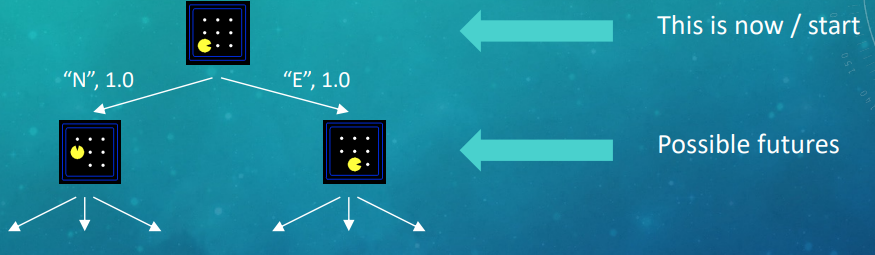
\includegraphics[width = 1\linewidth]{Images/14.PNG}
\end{center}
Invece di usare un albero per rappresentare il problema di ricerca, potremmo invece usare un \textbf{grafo dello spazio degli stati}: esso da una rappresentazione matematica del problema di ricerca nel seguente modo:
\begin{itemize}
    \item I nodi sono \textbf{le possibili configurazioni del mondo}
    \item Gli archi rappresentano \textbf{i risultati delle azioni}
    \item La funzione \textbf{"goal test"} viene rappresentata da un \textbf{insieme di nodi}
\end{itemize}
\begin{center}
    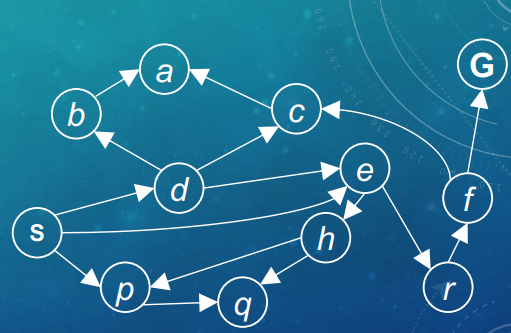
\includegraphics[width = 0.50\linewidth]{Images/15.PNG}
\end{center}
In un grafo dello spazio degli stati, \textbf{ogni stato occorre solamente una volta!} Tuttavia, raramente possiamo costruire l'intero grafo in memoria, poiché \textbf{esso cresce troppo velocemente}; tuttavia è un'idea utile.
Qual'è quindi la differenza sostanziale tra un grafo dello spazio degli stati e un albero di ricerca? Ogni \textbf{nodo} in un albero di ricerca è l'equivalente di un \textbf{intero cammino sul grafo dello spazio degli stati}.
Entrambi devono essere costruiti \textbf{"on demand"} (cioè li espandiamo solamente quando occorre) e devono esser espansi il meno possibile.
\subsubsection{Agenti basati su un'utilità e un modello}
\begin{center}
    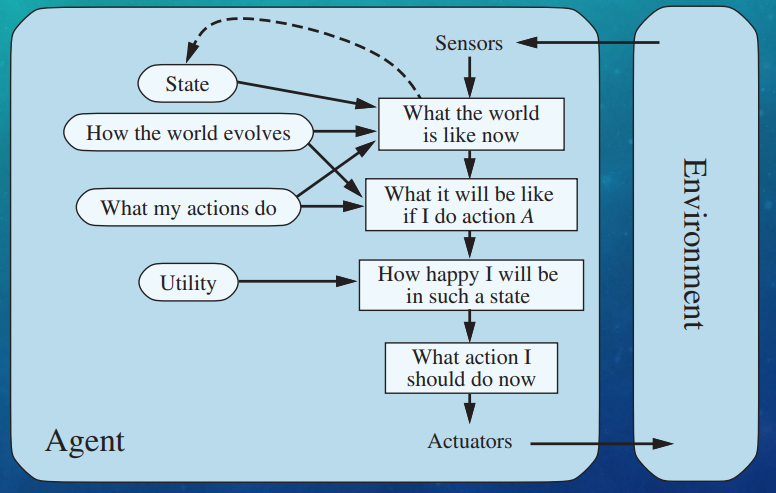
\includegraphics[width = 0.80\linewidth]{Images/16.PNG}
\end{center}
La differenza di questo tipo di agente con il precedente è la \textbf{scomparsa della funzione "goal test"} e l'introduzione di una \textbf{funzione "Utility"}, la quale è una vera e propria funzione
che attribuisce ad un certo stato del mondo un idea di \textbf{quanto quello stato sia desiderabile dall'agente}. Perché? Ci sono diversi motivi:
\begin{itemize}
    \item Potrei non essere in grado di definire formalmente una funzione che descriva l'obbiettivo
    \item Dato lo stato dell'ambiente, posso definire una funzione che valuti i vari elementi di esso e mi permetta di effettuare valutazione sulla prossima aziona da eseguire (es. scacchi)
    \item Avere una funzione d'utilità mi permette di considerare obbiettivi contrastanti fra loro; quindi poter definire una funzione che valuti tutti i fattori in gioco e che possa portare alla \textbf{discriminazione di certi stati} (es. problema di logistica)
\end{itemize}
\subsubsection{Caratteristiche dell'ambiente}
Russel e Norvig definiscono una serie di caratteristiche per l'ambiente:
\begin{itemize}
    \item \textbf{Ambienti accessibili vs Inaccessibili}: Un \textbf{ambiente accessibile} è un ambiente dove l'agente può ottenere un informazione \textbf{completa, accurata e aggiornata} riguardo lo stato dell'ambiente.
    Molti ambiente moderatamente complessi (includendo, per esempio, il mondo fisico e internet) sono \textbf{inaccessibili}. Più un ambiente è accessibile, più è semplice costruire un agente che possa operare in esso.
    I problemi di accessibilità del mondo si presentano ogni qualvolta che ci accingiamo a risolvere problemi nel \textbf{mondo fisico}
    \item \textbf{Ambienti deterministici vs non-deterministici}: Un \textbf{ambiente deterministico} è un ambiente in cui ogni azione ha un singolo effetto garantito: non c'è \textbf{incertezza} riguardo allo stato in cui l'ambiente si troverà in seguito al compiersi di un azione. Il mondo fisico dovrebbe essere sempre considerato come sostanzialmente \textbf{non-deterministico}, salvo certi casi in cui si può pensare come deterministico.
    Gli ambienti non-deterministici presentano problemi maggiore per il progettista dell'agente.
    \item \textbf{Ambienti episodici vs sequenziali}: In un ambiente \textbf{episodico}, l'esperienza dell'agente può essere divisa in \textbf{passi atomici} dove l'agente percepisce uno stimolo ed effettua una singola azione. La scelta dell'azione da intraprendere \textbf{dipende solamente dall'episodio stesso}.
    Gli ambienti episodici sono più semplici dal punto di vista del progettista dell'agente, poiché l'agente può decidere quale azione intraprendere basandosi solo sull'episodio corrente, \textbf{non deve quindi ragionare riguardo all'interazione tra questo episodio e quelli futuri}.
    \item \textbf{Ambienti statici vs dinamici}: Per \textbf{ambiente statico} si intende un ambiente che \textbf{non cambia nel mentre che l'agente sta decidendo l'azione da compiere}; un cambiamento in un ambiente statico avviene quindi \textbf{solamente a causa di un'azione da parte dell'agente}.
    Per \textbf{ambiente dinamico} si intende un ambiente che \textbf{cambia mentre l'agente sta decidendo quale azione intraprendere} e che quindi ha al suo interno altri processi, oltre all'agente, che ne modificano lo stato e le cui azioni possono interferire con le azioni dell'agente (come nella teoria dei sistemi concorrenti); le trasformazioni di un ambiente dinamico quindi avvengono \textbf{al di fuori del controllo dell'agente}.
    Il mondo fisico è un ambiente altamente dinamico.
    \item \textbf{Ambienti discreti vs continui}: Un \textbf{ambiente discreto} è un ambiente che presenta un numero \textbf{fissato e finito} di azioni e di percezioni in esso. Gli \textbf{ambienti continui} hanno un certo livello di \textbf{discrepanza} con i sistemi computerizzati.
    Gli ambienti discreti potrebbero essere gestiti, in linea di principio, da una specie di \textbf{tabella di ricerca} (lookup table).
    Per semplificare la gestione di un ambiente continuo, si può \textbf{sovrapporre ad esso una sua discretizzazione} in modo da rendere più semplice la progettazione e l'implementazione degli agenti che devono operare al suo interno.
\end{itemize} 
\begin{center}
    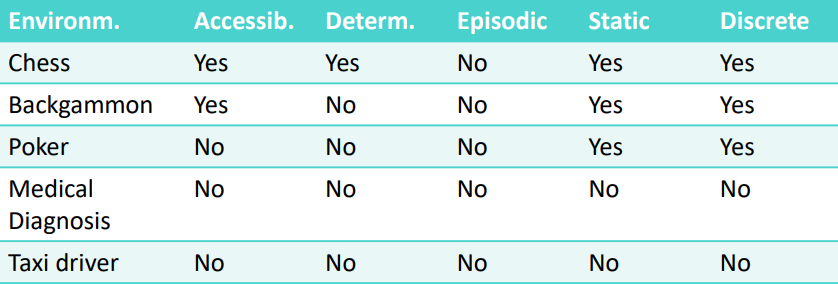
\includegraphics[width = 0.80\linewidth]{Images/17.PNG}
\end{center}



\end{document}